\documentclass[a4paper,12pt,twocolumn]{article}

\usepackage{cite} 
\usepackage{natbib}
\usepackage{amsmath}
\usepackage{amssymb}
\usepackage{graphicx}
\usepackage{caption}
\usepackage{subcaption}
\usepackage{algorithm}
\usepackage{algpseudocode}
\usepackage{listings}
\usepackage{booktabs}
\usepackage{siunitx}
\usepackage{enumitem}


\date{ }
\title{An In-Depth Analysis of \\ Selection Sort \& Insertion Sort}
\author
{
\begin{tabular}[t]{c@{\extracolsep{9mm}}c@{\extracolsep{9mm}}c}
{\it Md. Barkullah} & {\it Partha Paul} & {\it Md. Abu Sufyan}\\
{\small Dept. of CSE} & {\small Dept. of CSE} & {\small Dept. of CSE}\\
{\small RUET} & {\small RUET} & {\small RUET}\\
{\small 2003071@student.ruet.ac.bd} & {\small 2003078@student.ruet.ac.bd} & {\small 2003085@student.ruet.ac.bd}\\
\\
{\it Md. Tameem Rahman} & {\it Mir Ashikur Rahman} & {\it Md. Atik Mouhtasim}\\
{\small Dept. of CSE} & {\small Dept. of CSE} & {\small Dept. of CSE}\\
{\small RUET} & {\small RUET} & {\small RUET}\\
{\small 2003089@student.ruet.ac.bd} & {\small 2003109@student.ruet.ac.bd} & {\small 2003118@student.ruet.ac.bd}\\
\end{tabular}
}






\begin{document}
\maketitle

\begin{abstract}
    The ordering of numbers in an integer array in computer science and mathematics is one of the most important topics. For this purpose, there are a large variety of sorting algorithms like Selection sort, Insertion sort, Quick sort, Radix sort, Merge sort and Bubble sort. Sorting algorithms play a crucial role in organising data efficiently, and two widely used techniques are Insertion Sort and Selection Sort.  In this study, two sorting algorithms are investigated as Selection and Insertion sort. This study compares performance of Selection sort and Insertion sort algorithms that are used commonly in terms of running time.
\end{abstract}


\section{Introduction}

Sorting process in data structure is essential for transforming randomly distributed elements into either decreasing or ascending order. Various sorting algorithms, including Selection sort, Insertion sort, Quick sort, and Radix sort, have been developed to reduce complexity and enhance the performance of sorting.

In this study, the focus is on comparing the Selection sort and Insertion sort algorithms in terms of their running time. The following sections provide an in-depth explanation of the Selection sort algorithm, its working logic illustrated with an example, and its implementation in the C++ programming language. Additionally, the running time for sorting using the Selection sort algorithm is presented.\cite{furat2016comparative}

Subsequently, the Insertion sort algorithm is introduced, along with its working logic demonstrated through an example. The code for the Insertion sort algorithm is implemented in the C++ programming language, and the running time for sorting using this algorithm is provided.

Finally, a comparative analysis of the Selection sort and Insertion sort algorithms is presented, focusing on their time complexity.

%

\section{Background Study}


\subsection{Selection Sort:}
Selection sort is a simple comparison-based sorting algorithm. The algorithm begins by finding the smallest element in the array and then exchanges this smallest element with the element in the first position. After this initial step, the algorithm proceeds to select the smallest element in the unsorted part of the array in each step of the sorting process. It exchanges this selected smallest element with the element in the unsorted part of the current step. This process continues until there are no unsorted elements remaining in the array. Notably, the selection sort algorithm spends a significant amount of time finding the smallest element in the unsorted part of the array.
\subsubsection*{Work Logic of the Selection Sort Algorithm}
\textbf{First Pass:}
\begin{itemize}
    \item For the first position in the sorted array, the entire array is traversed sequentially from index 0 to 4. The element at the first position is replaced with the smallest value found during traversal.
    \item After one iteration, the least value (in this case, 8) appears in the first position of the sorted list and 72 is placed at the position where 8 was originally placed in.
\end{itemize}
\begin{center}
    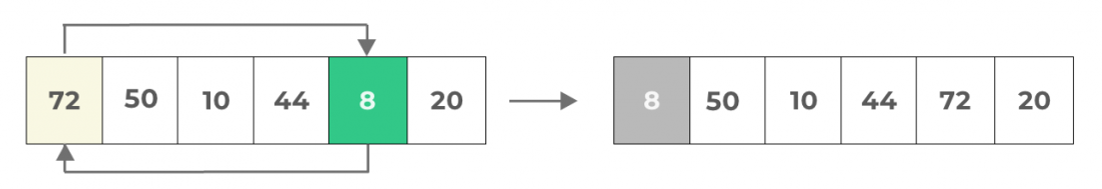
\includegraphics[width=0.9\linewidth]{pass-1.png}
    \label{pass-1}
\end{center}
\textbf{Second Pass:}
\begin{itemize}
    \item For the second position, where 50 is present, the rest of the array is traversed in a sequential manner.
    \item After traversing, it is determined that 10 is the second lowest value in the array, and it should appear at the second place in the array. Thus, these values are swapped.
\end{itemize}
\begin{center}
    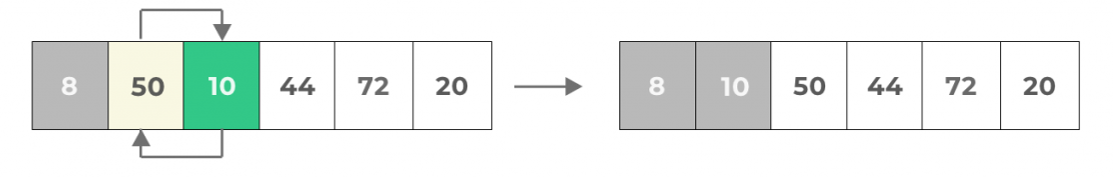
\includegraphics[width=0.9\linewidth]{pass-2.png}
    \label{pass-2}
\end{center}
\textbf{Third Pass:}
\begin{itemize}
    \item For the third position, where 50 is present again, the rest of the array is traversed to find the third least value present in the array.
    \item While traversing, 20 is identified as the third least value, and it should appear at the third place in the array. Thus, a swap is performed between 20 and the element present at the third position.
\end{itemize}
\begin{center}
    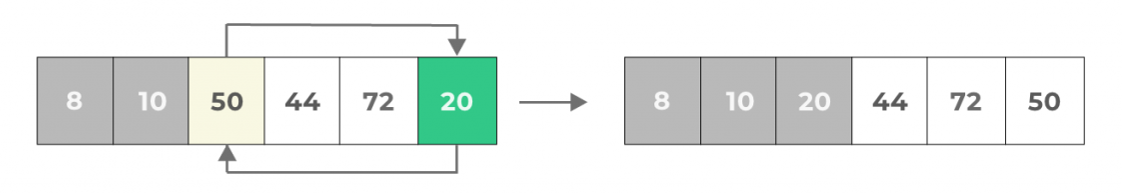
\includegraphics[width=0.9\linewidth]{pass-3.png}
    \label{pass-3}
\end{center}
\textbf{Fourth Pass:}
\begin{itemize}
    \item Similarly, for the fourth position, the rest of the array is traversed to find the fourth least element in the array.
    \item As 44 is the fourth lowest value, it is placed at the fourth position.
\end{itemize}
\begin{center}
    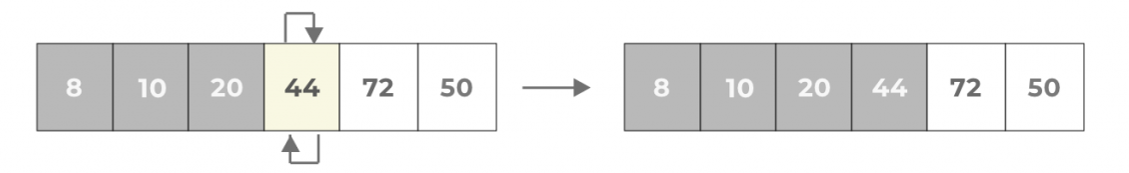
\includegraphics[width=0.9\linewidth]{pass-4.png}
    \label{pass-4}
\end{center}
\textbf{Fifth Pass:}
\begin{itemize}
    \item At last,for the position where 72 is hold the array is traversed onwards and 50 is found the next least valued number and is swapped with 72.
    \item As there is onle one element left the resulting array is the sorted array becouse that last element is already at the right position according to its value.
\end{itemize}
\begin{center}
    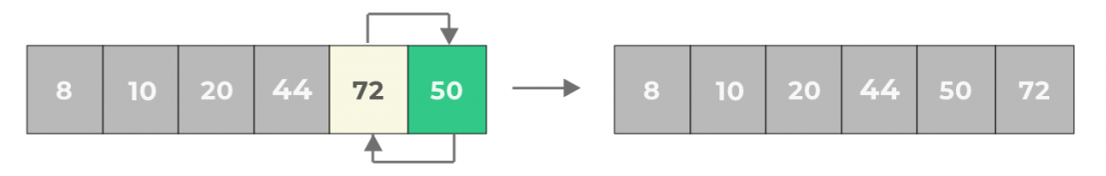
\includegraphics[width=0.6\linewidth]{pass-5.png}
    \label{pass-5}
\end{center}

\begin{figure}[H]
    \centering
    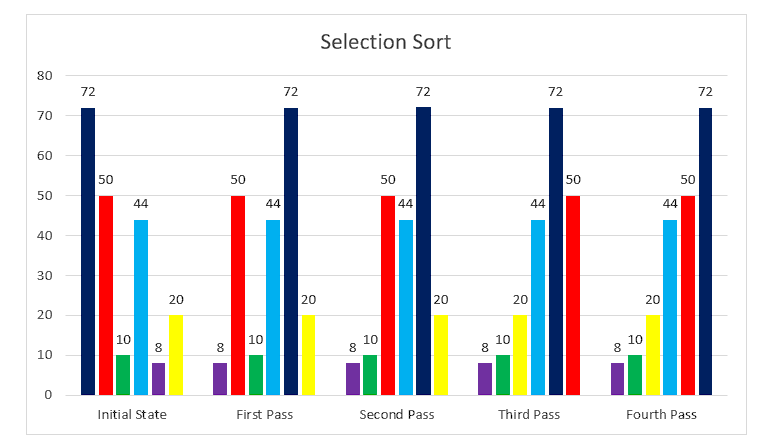
\includegraphics[width=\linewidth]{chart1.png}
    \captionsetup{font=small, textfont=it}
    \caption*{Chart 1 : Selection sort algorithm passes}
    \label{fig:chart1}
\end{figure}

\begin{algorithm}[H]
    \caption{: Selection Sort\cite{horowitz1997computer}}
    \begin{algorithmic}[1]
    \For{$i \gets 1$ to $n-1$}
        \State $smallest \gets i$
        \For{$k \gets i+1$ to $n$}
            \If{$arr[k] < arr[min]$}
                \State $min \gets k$
            \EndIf
        \EndFor
        \State Swap $arr[min]$ and $arr[j]$
    \EndFor
    \end{algorithmic}
\end{algorithm}

\textbf{Loop Invariant:}
At the start of each iteration of the $for$ loop of lines 1 - 9, the subarray $arr[0..i-1]$ is always sorted.\cite{geeksforgeeks}


\subsection{Insertion Sort:}

Insertion sort is a simple comparison-based sorting algorithm. The algorithm starts by comparing the first two elements in the array. If the first element is greater than the second element, they are exchanged. This process is then implemented for all neighboring indexed elements.
\\ \\
Consider an example:\\
\begin{center}
    \(\text{arr[]} = \{23, 1, 10, 5, 2\}\)
\end{center}

Suppose \(n\) is the number of elements in the array. For example, consider an integer array with 5 elements, so \(n\) is 5 for this sample, and sorting of this integer array in ascending order is desired:
\\
%
\subsubsection*{Work Logic of the Insertion Sort Algorithm}
\hspace{2.7mm}
\textbf{First Pass:}
\begin{itemize}
    \item The first item of the array is always sorted as there is no value to compare it with so relative to itself it is already sorted.
\end{itemize}
\begin{center}

    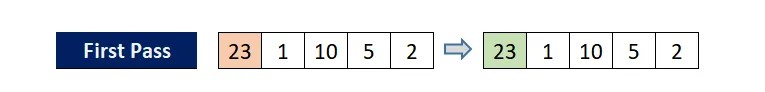
\includegraphics[width=\linewidth]{pass1.jpg}
    \label{fig:pass1}
\end{center}
\textbf{Second Pass:}
\begin{itemize}
    \item Now iterate to the 2nd element and compare with the first element.
    \item Here, 23 is greater than 1; hence, they are not in ascending order, and 23 is not at its correct position. Thus, swap 1 and 23.
    \item So, for now, 1 is stored in a sorted sub-array where 23 is in the 2nd position and 1 is at first.
\end{itemize}
\begin{center}
    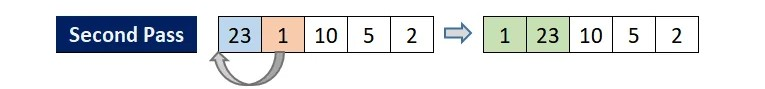
\includegraphics[width=\linewidth]{pass2.jpg}
    \label{fig:pass2}
\end{center}
\textbf{Third Pass:}
\begin{itemize}
    \item Now, move to the next two elements and compare them.
    \item Here, 10 is compared to 23, and as 23 is greater, a swap operation is performed.
    \item Then, 10 is compared with 1, and as 1 is smaller, no swapping occurs. Resulting in a partially sorted array.
\end{itemize}
\begin{center}
    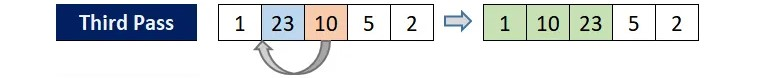
\includegraphics[width=\linewidth]{pass3.jpg}
    \label{fig:pass3}
\end{center}
\textbf{Fourth Pass:}
\begin{itemize}
    \item Now, comparison starts with 5 and 23, which results in swapping as 5 is smaller and is at a higher position in the array.
    \item After the swap, 5 is compared to 10 and is again swapped with 10, getting to the 2nd position in the array.
    \item Then, 5 is compared with 1 and is not swapped, resulting in a partially sorted array.
\end{itemize}
\begin{center}
    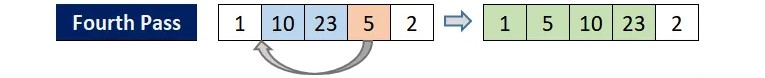
\includegraphics[width=\linewidth]{pass4.jpg}
    \label{fig:pass4}
\end{center}
\textbf{Fifth Pass:}
\begin{itemize}
    \item Now, the elements 1, 5, 10, 23 are sorted with respect to each other, leaving only 2.
    \item Comparison starts from 2 with 23, and as 23 is greater than 2, a swap operation is performed.
    \item This comparison and swapping continue until 2 reaches the 2nd position, as 10 and 5 are both greater than 2.
    \item As 1 is smaller than 2, no swap operation is performed, and the result is the complete sorted array.
\end{itemize}
\begin{center}
    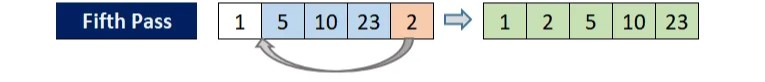
\includegraphics[width=\linewidth]{pass5.jpg}
    \label{fig:pass5}
\end{center}
Hence, the sorted array is:
\begin{center}
    \(\text{arr[]} = \{1, 2, 5, 10, 23\}\)
\end{center}

\begin{figure}[!hbt]
    \centering
    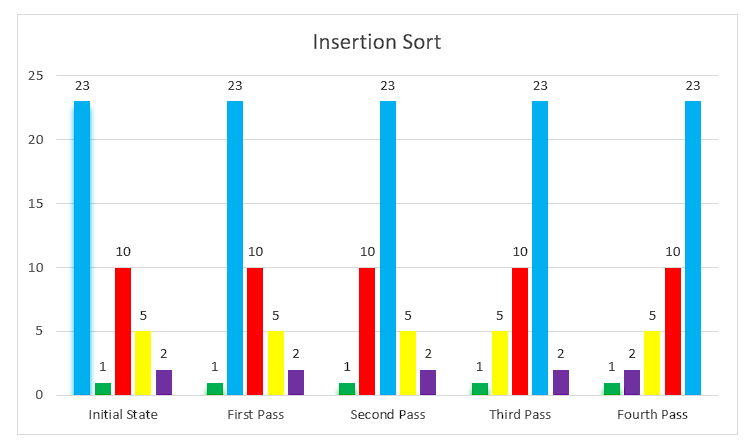
\includegraphics[width=\linewidth]{chart2.png}
    \captionsetup{font=small, textfont=it}
    \caption*{Chart 2 : Selection sort algorithm passes}
    \label{fig:chart2}
\end{figure}



\begin{algorithm}[H]
    \caption{: Insertion Sort\cite{cormen2022introduction}}
    \begin{algorithmic}[1]
    \For{$j \gets 2$ to $Arr.lenght$}
    \State $key = Arr[j]$
    \State $i = j- 1$
        \While{$i>0$ and $Arr[i]>key$}
                \State $Arr[i+1]=Arr[i]$
                \State $i=i-1$
        \EndWhile
        \State $Arr[i+1]=key$
    \EndFor
    \end{algorithmic}
\end{algorithm}
\quad\\
\textbf{Loop Invariant:}
At the start of each iteration of the $for$ loop of lines 1 - 9, the subarray $Arr[1..j-1]$ consists of the elements originally in $Arr[1..j-1]$,but in sorted order.\cite{cormen2022introduction}


\section{Results and Analysis}
\subsection*{Time Complexity:}
\begin{itemize}[label=--]
    \item \textbf{Selection Sort:} The time complexity of Selection Sort is \(O(n^2)\) in the worst and average cases. This is because, for each element, it needs to traverse the remaining unsorted part of the array to find the minimum element and swap it with the current element.
    \item \textbf{Insertion Sort:} The time complexity of Insertion Sort is also \(O(n^2)\) in the worst and average cases. It involves iterating through the array and inserting each element into its correct position by comparing it with the elements to its left.
\end{itemize}
\subsection*{Best-Case Scenario:}
\begin{itemize}[label=--]
    \item \textbf{Selection Sort:} The best-case time complexity of Selection Sort is \(O(n^2)\). Even if the array is partially sorted, Selection Sort still needs to traverse the entire unsorted part for each element.
    \item \textbf{Insertion Sort:} The best-case time complexity of Insertion Sort is \(O(n)\) when the array is already sorted. In such cases, it only needs to compare each element with its adjacent element to verify the order.
\end{itemize}
\begin{table}[H]
    \centering
    \small
    \captionsetup{font=small, textfont=it}
    \label{tab:sort-comparison}
    \begin{tabular}{@{}S[table-format=6.0]SS[table-format=3.6]S[table-format=3.6]@{}}
        \toprule
        \textbf{Size} & \textbf{Insertion (s)} & \textbf{Selection (s)} \\
        \midrule
        10 & 0.000011 & 0.000019 \\
        50 & 0.000176 & 0.000155 \\
        100 & 0.000412 & 0.000363 \\
        500 & 0.004555 & 0.004457 \\
        1000 & 0.020648 & 0.018857 \\
        5000 & 0.528669 & 0.485517 \\
        10000 & 2.105405 & 1.965638 \\
        50000 & 55.541591 & 61.877976 \\
        100000 & 238.821475 & 271.276342\\
        \bottomrule
    \end{tabular}
    \captionsetup{font=small, textfont=it}
    \caption{Performance Comparison of Insertion Sort and Selection Sort}
\end{table}
\begin{figure}[H]
    \centering
    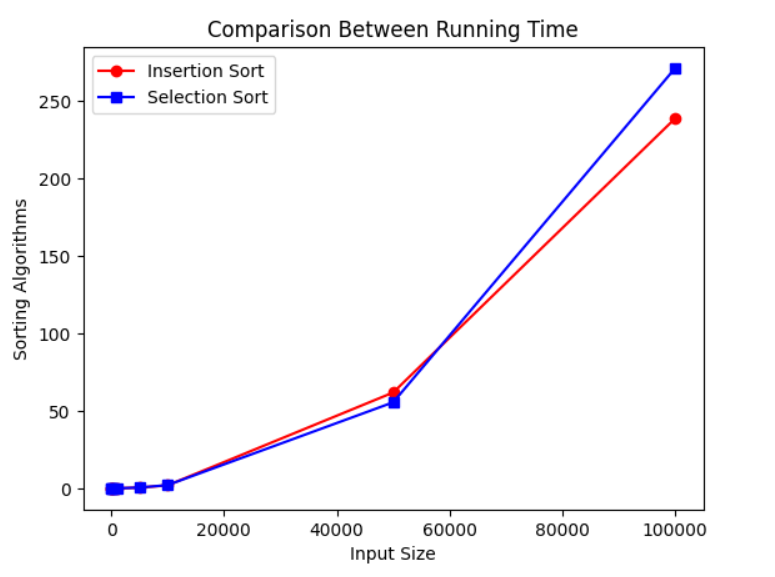
\includegraphics[width=\linewidth]{graph-1.png}
    \label{fig:graph-1}
    \captionsetup{font=small, textfont=it}
    \caption*{Graph 1 : Running time comparison of Insertion Sort and Selection Sort}
\end{figure}




\subsection*{Interpretation of the Graph:}
\begin{itemize}
    \item As the dataset size increases, the running time of both algorithms tends to increase, which is expected for sorting algorithms with quadratic time complexity.
    \item The lines illustrate the trend of how the runtime increases with the size of the input data.
    \item For smaller dataset sizes, Insertion Sort might perform better than Selection Sort. However, as the dataset size increases, Selection Sort may start to perform relatively better than Insertion Sort.
\end{itemize}



\section{Conclusion}

We compared insertion sort and selection sort to assess their performance across varying amounts of data, with a focus on understanding how their efficiency changes with different dataset sizes.

Our findings indicate that insertion sort tends to outperform selection sort on small datasets, especially when dealing with data that is already well-sorted. However, as the dataset size increases, selection sort emerges as a strong candidate due to potential efficiency benefits. This observation may be attributed to the decreasing constant factor in time complexity.

This comparative analysis provides insights into the strengths and weaknesses of these sorting methods. While both insertion sort and selection sort have their merits, the choice should be based on the specific characteristics of the data and the scale of the sorting task.

We acknowledge certain limitations in our study, including a focus on worst and average scenarios and an assumption of a uniform distribution for random data generation. This opens avenues for future research to explore the real-world effects of these algorithms and discover ways to enhance their capabilities. In summary, our study contributes to a deeper understanding of sorting algorithms, offering valuable insights for decision-making when selecting algorithms for diverse applications.

Examining insertion and selection sorts not only enhances comprehension of their inner workings but also stimulates ongoing efforts to optimize the sorting process for various computational situations.

\nocite{*}
\bibliographystyle{plain}
\bibliography{Bibliography1}

\end{document}
